\chapter{Using color separation as a stellar characterization tool}\label{chap:4}
% TEXT ==========================================

In this chapter, we consider the scope of using color as a stellar characterization tool. We display the probability functions and color statistics from our data analysis in Chapter \ref{chap:3}. We discuss how colors \jwone and \jwtwo, which showcase dwarf-giant separation, can be used in upcoming and current large-scale astronomical surveys, and the viability of using color as a characterization tool.

\section{Color probability density functions} \label{sec:color_prob_func}

From Chapter \ref{chap:3}, we have a method of determining color likelihood given a specified spectral and luminosity class. We can inversely use this color-luminosity-spectral class relationship to predict luminosity classes in cases that color and spectral class 
is known. In this section we present the probability density functions derived from fitting to Student's t-distribution in Chapter \ref{subsec:tdist_stats}, and is visualized in Figures \ref{fig:periodic-pdf-jw1},  \ref{fig:periodic-pdf-jw2}, \ref{fig:periodic-delta-jw1}, and \ref{fig:periodic-delta-jw2}. We note that the color separation is subtle but non-negligible, on the order of $\sim$0.10 and $\sim$0.14 magnitudes for \jwone and \jwtwo, respectively, for spectral types G0--K3. No significant difference is observed for other spectral sub-types.

Figures \ref{fig:periodic-pdf-jw1} and \ref{fig:periodic-pdf-jw2} displays probability functions that are dependent on photometric color, spectral type, and luminosity class group (dwarfs and giants), from fitting photometric data to a Student's t-distribution. There is a separation between dwarf and giant colors among spectral types G0 to K3. Grayed plots signify a spectral-type bin for which we do have some data, but have fewer than 4 stars in either luminosity group and thus cannot calculated an average. Spectral types not listed at all are types that are not represented in our $\sim$20,000 cross-matched sample from photometric and spectral catalogs, a process is described in Chapter \ref{chap:2} and visualized in Figure \ref{fig:spt_michigan_hist}.

In order to get a clear idea of the where the maximum color separation occurs for a given spectral type, we produced a map of differences of the color averages for each spectral bin (Figures \ref{fig:periodic-delta-jw1} and \ref{fig:periodic-delta-jw2}). We have simply subtracted color of the peak probability (or the average) of giants from the dwarfs for each spectral subtype bin. Presumably, the greater the difference or separation in color, the easier it will be to differentiate giants from dwarfs of the same spectral type. Both plots help highlight the spectral types for which we see the most color difference, G to early K-type stars. The values of the color separation of giants from dwarfs and the color average for each spectral sub-type bin is also displayed in Appendix C, Table \ref{table:color_avgs}.

\section{Applicability to modern surveys}
In this section we address using color separation as a characterization tool for stars in the scope of modern surveys. We note the importance the $J$ band is in differentiating between dwarfs from giants given its previously proved sensitivity for differentiating M dwarfs from GK dwarfs for $J-K$. The combination of this study with $J-W_{1}$ and $J-W_{2}$ in being sensitive for GK dwarfs, and $J-K$ being sensitive for GKM stars suggests the presence of surface gravity sensitive lines in the $J$ band. Thus, there we suggest it is viable to search for gravity sensitive lines within the wavelength coverage of this photometric band. 


We consider use in large-scale  surveys that include photometric observations such as LAMOST, RAVE , or upcoming LSST. While color can help determine luminosity class, our tool would not work unless there is also a reliable estimate of spectral type as well, and enough of a sample size to constrain a possible color separation.

% FIGURES ==========================================
\begin{figure}
    \centering
    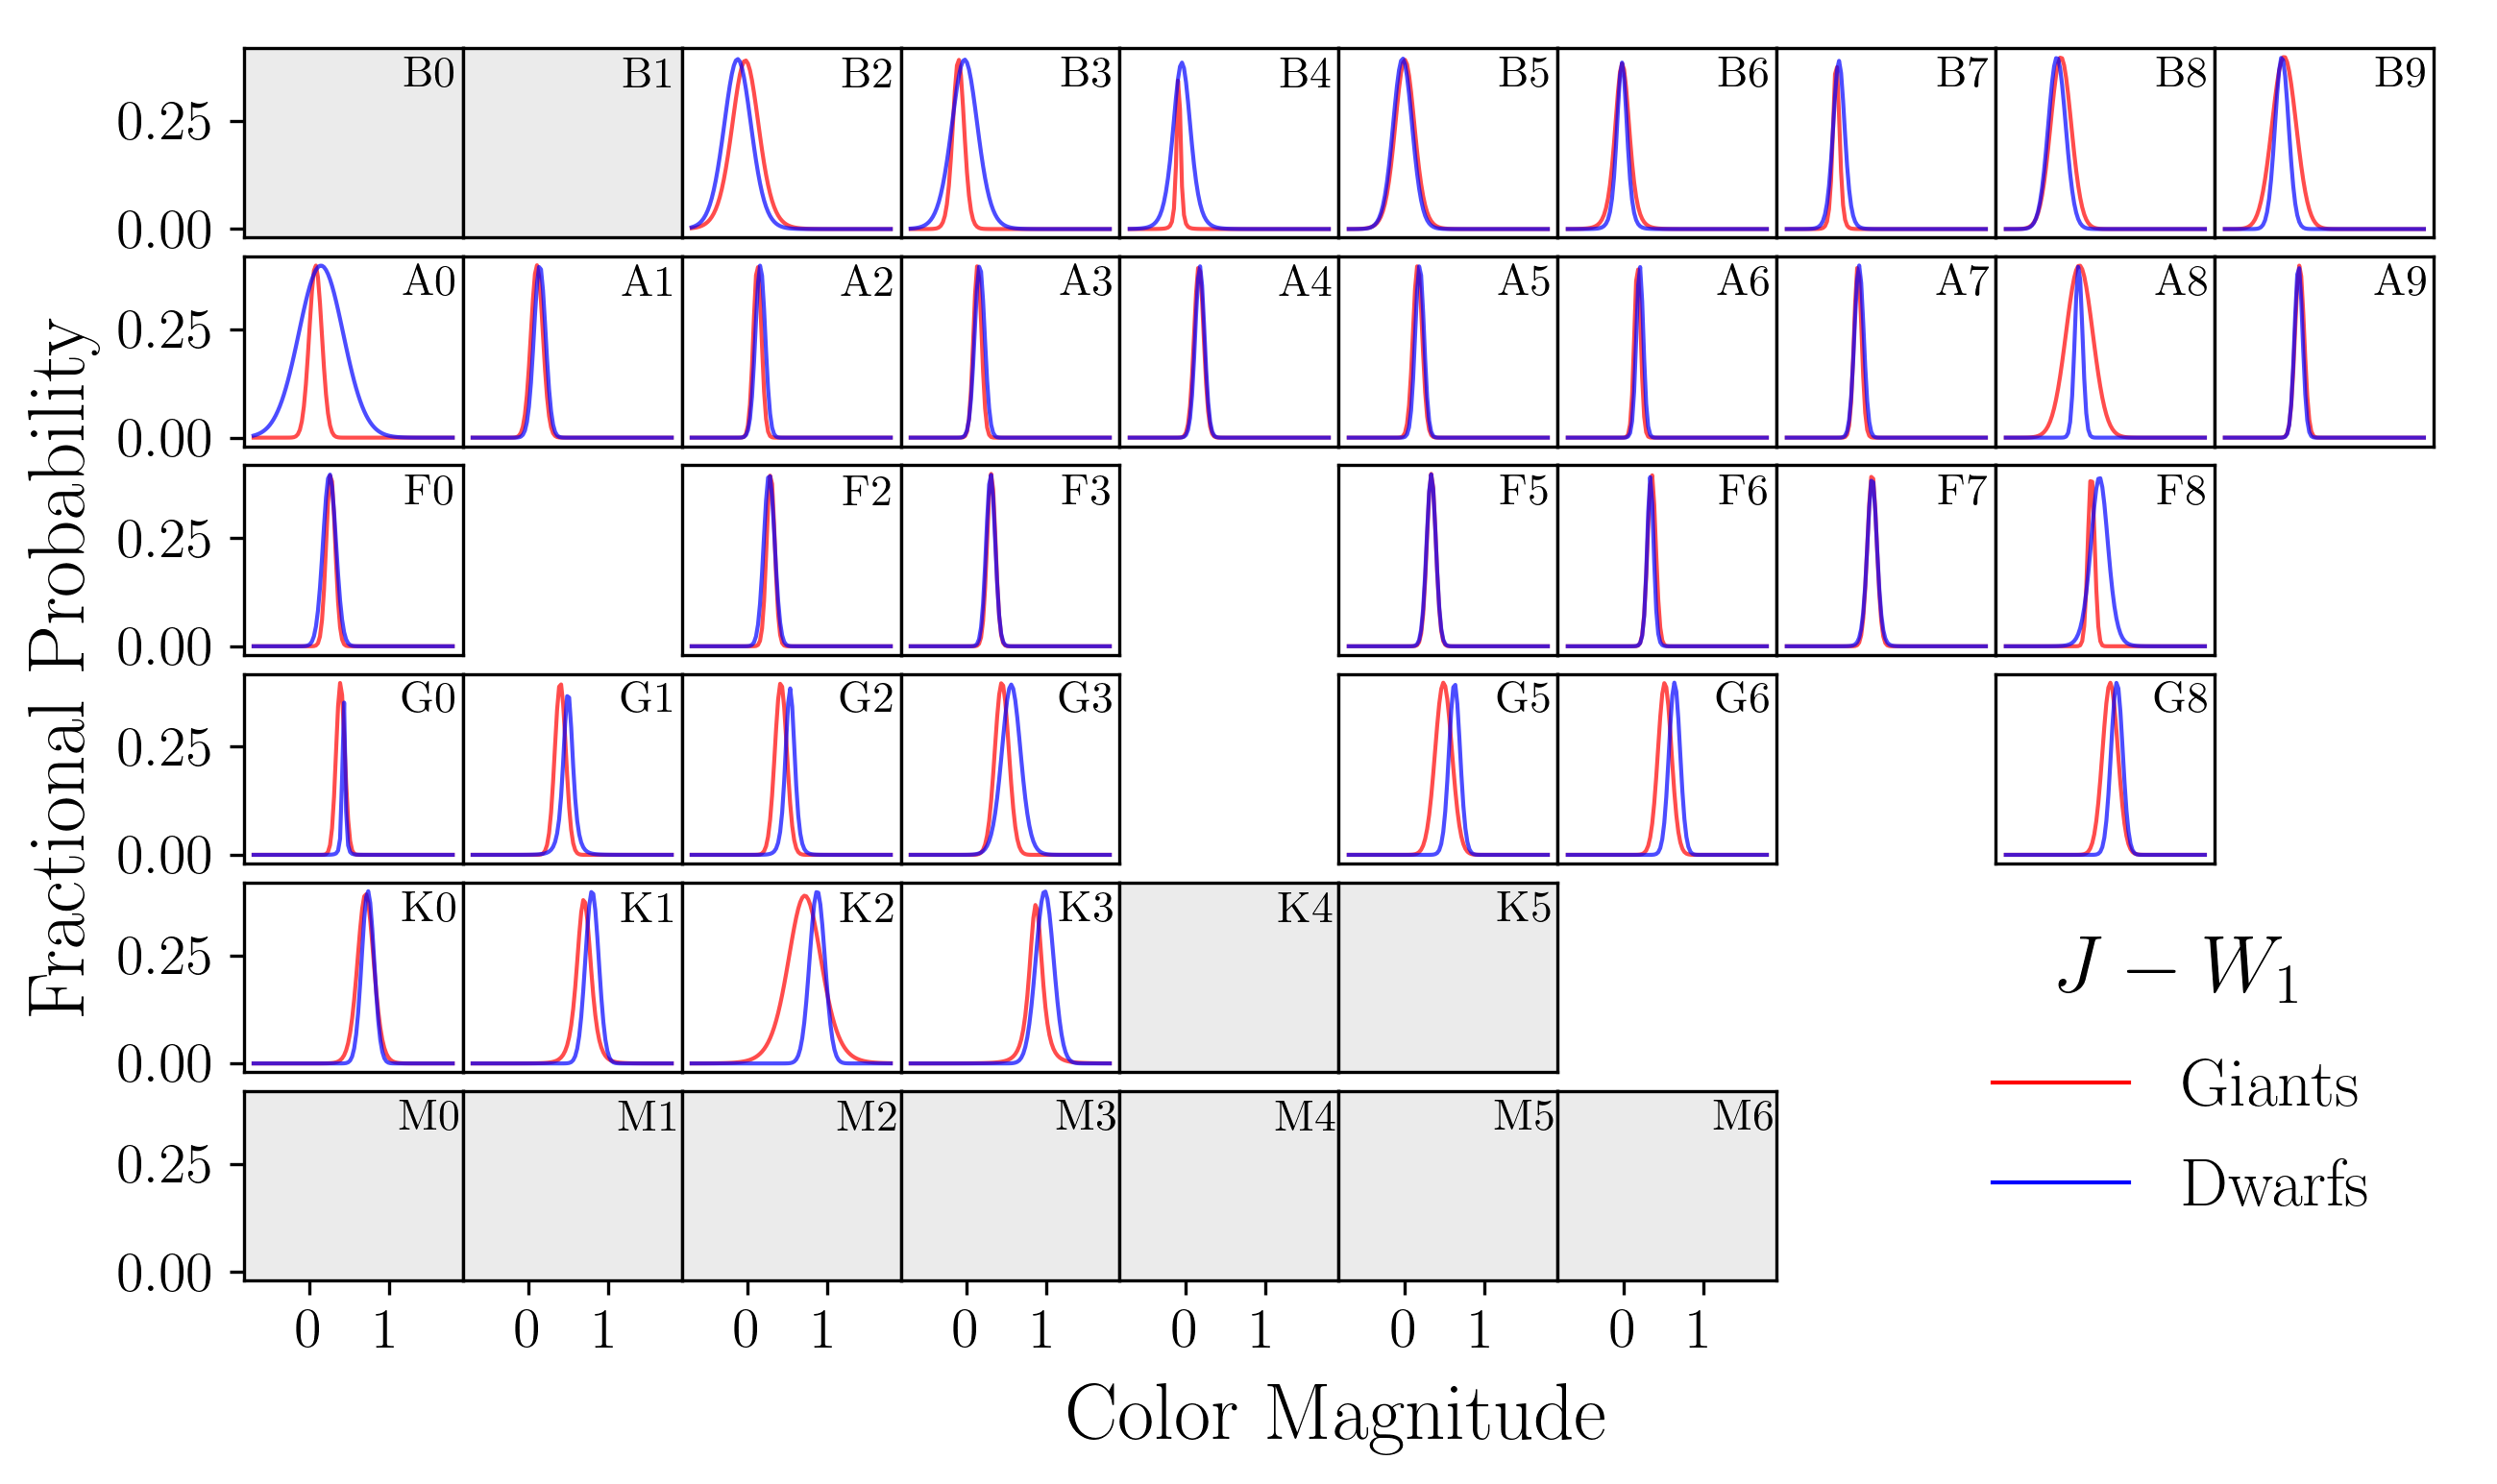
\includegraphics[width=1.0\textwidth,clip=true]{Figures/periodic/periodic-t-pdf_J_W1.png}
    \caption{This figure displays each available spectral subtype bin for which we could do color analysis. The curves represents color data fitted to a Student's t-distribution; red represents giants (luminosity classes I, II, III, and IV) and blue represents dwarfs (V). The color value for which the peak occurs in a the distribution is the average. Grayed areas are spectral sub-type bins for which we have photometric, spectral, and luminosity class data but not enough stars to conduct color analysis. See Chapter \ref{sec:color_prob_func} and \ref{subsec:tdist_stats} for more detailed discussion on how these statistical distributions were calculated.}
    \label{fig:periodic-pdf-jw1}
\end{figure}

\begin{figure}
    \centering
    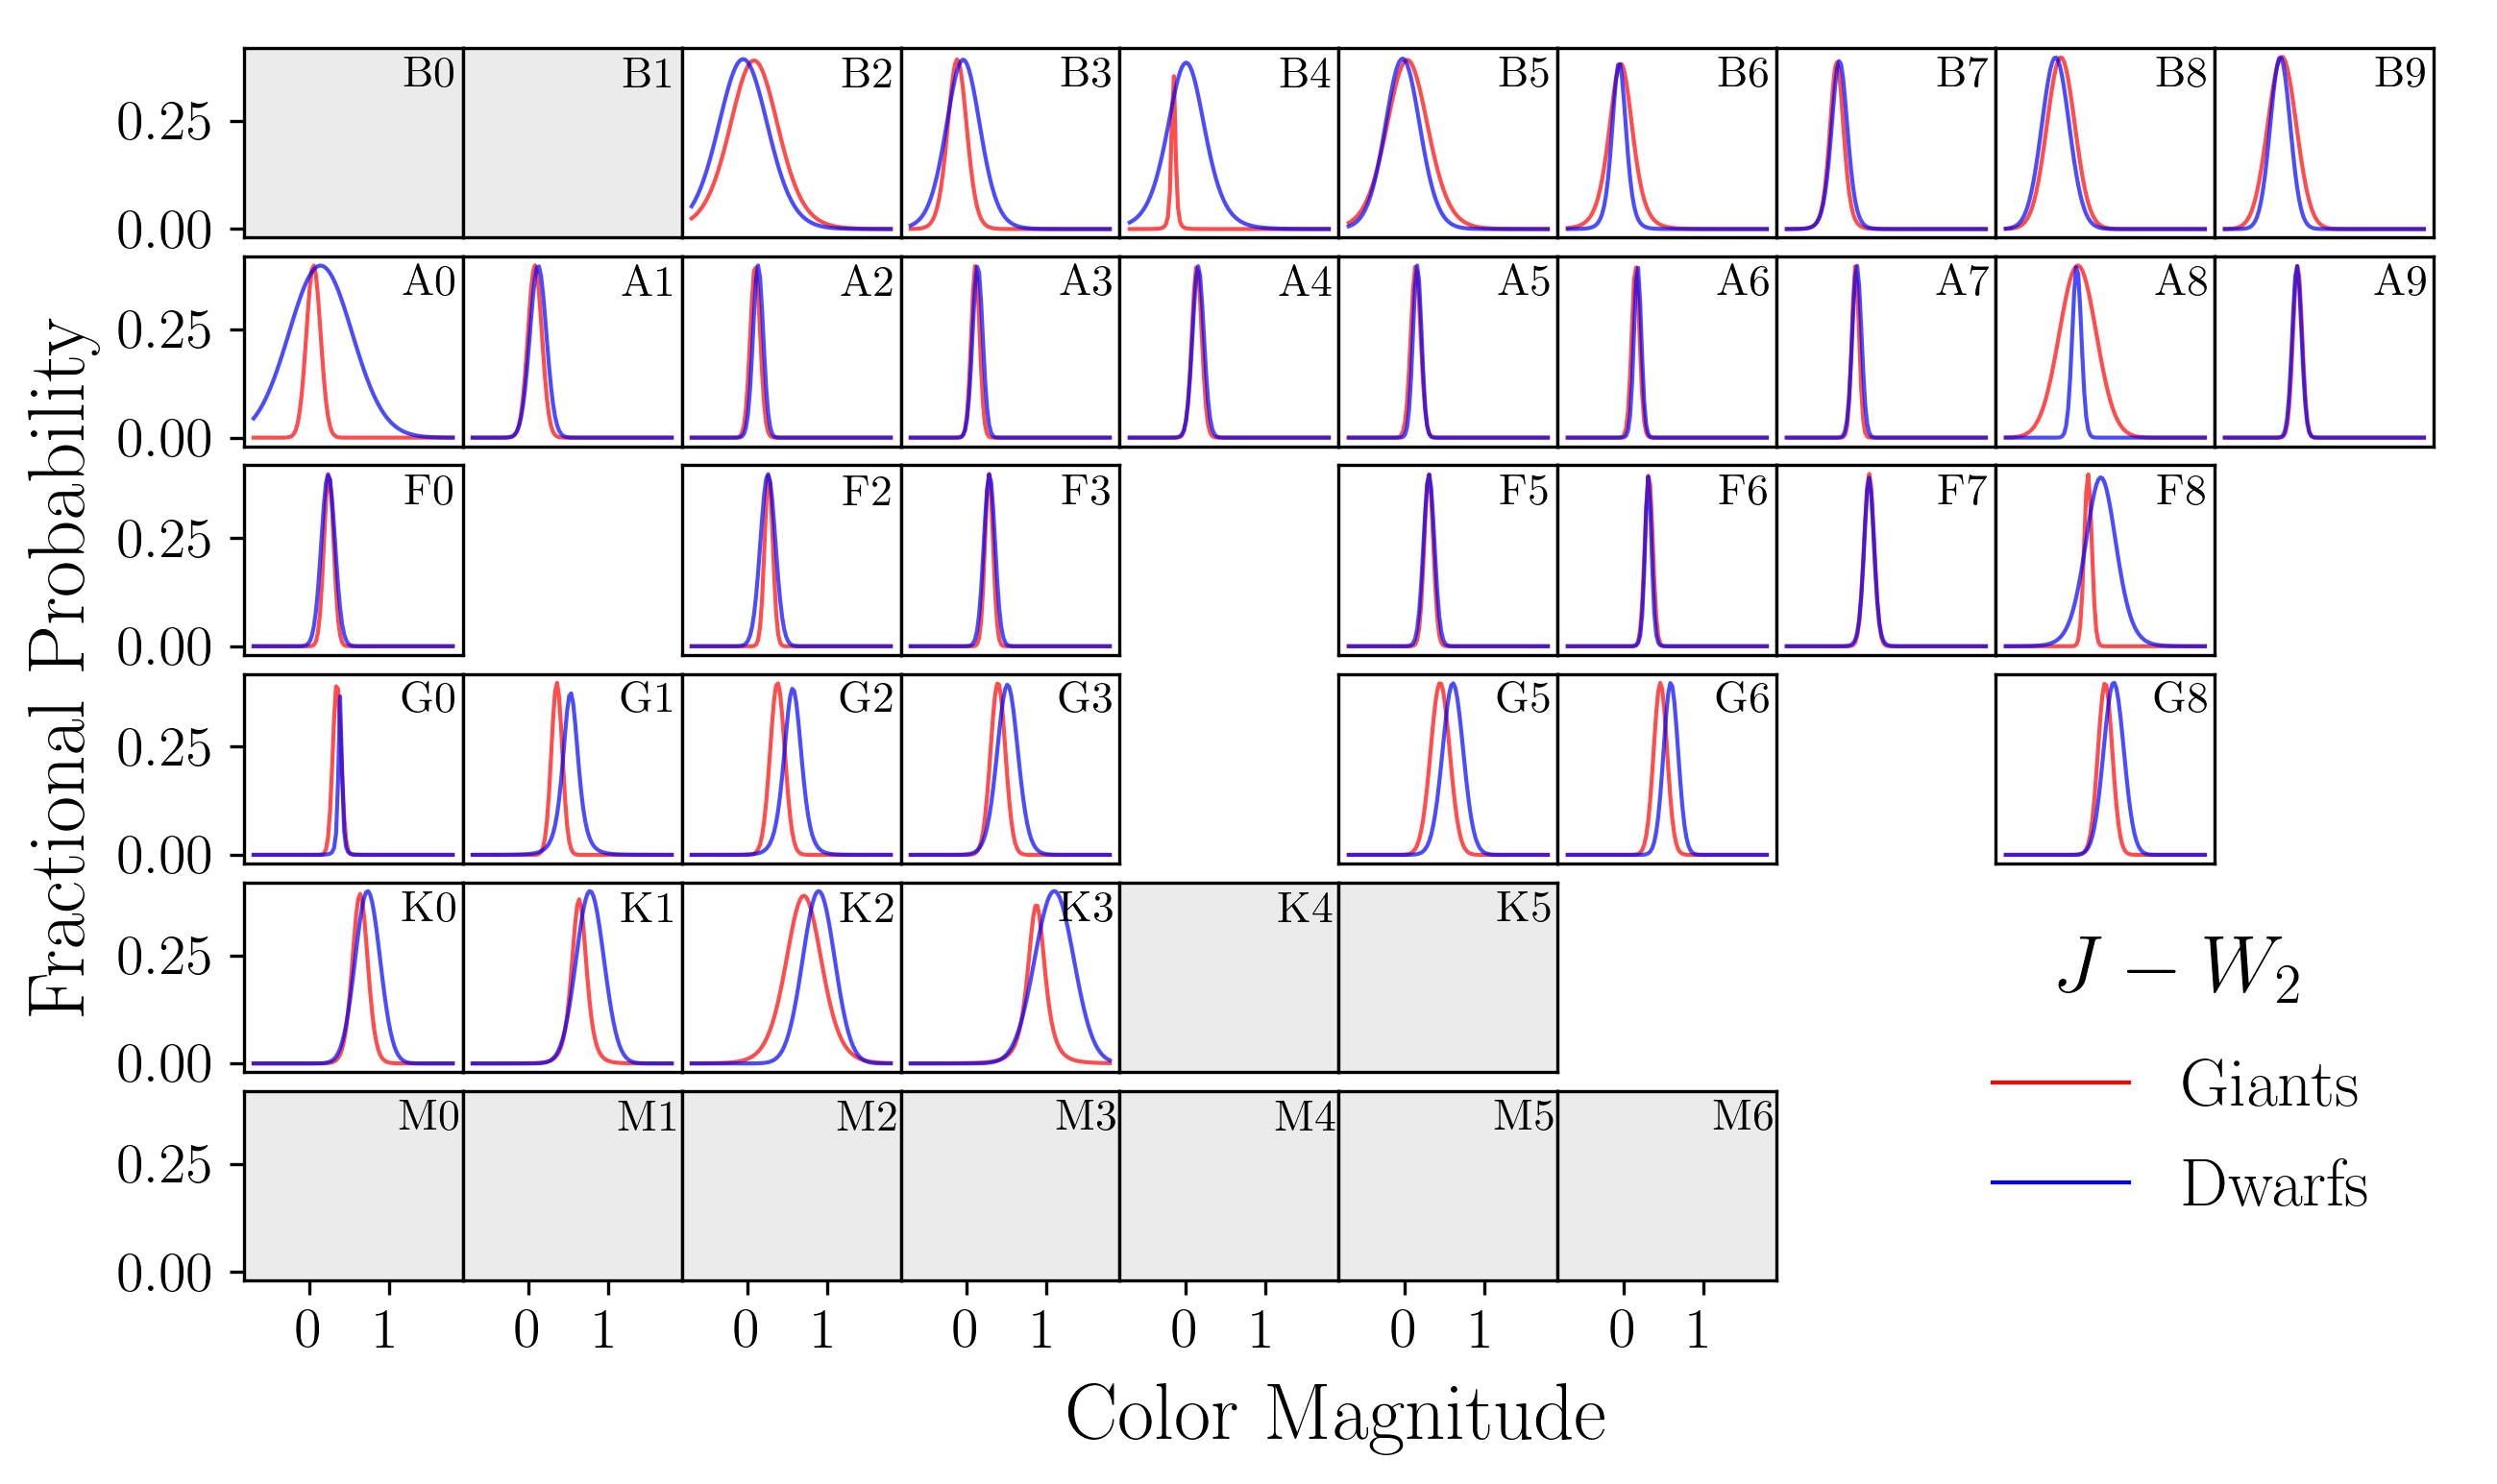
\includegraphics[width=1.0\textwidth,clip=true]{Figures/periodic/periodic-t-pdf_J_W2.png}
    \caption{Same as Figure \ref{fig:periodic-pdf-jw1}, but for $J-W_{2}$.}
    \label{fig:periodic-pdf-jw2}
\end{figure}
\clearpage
\begin{figure}
    \centering
    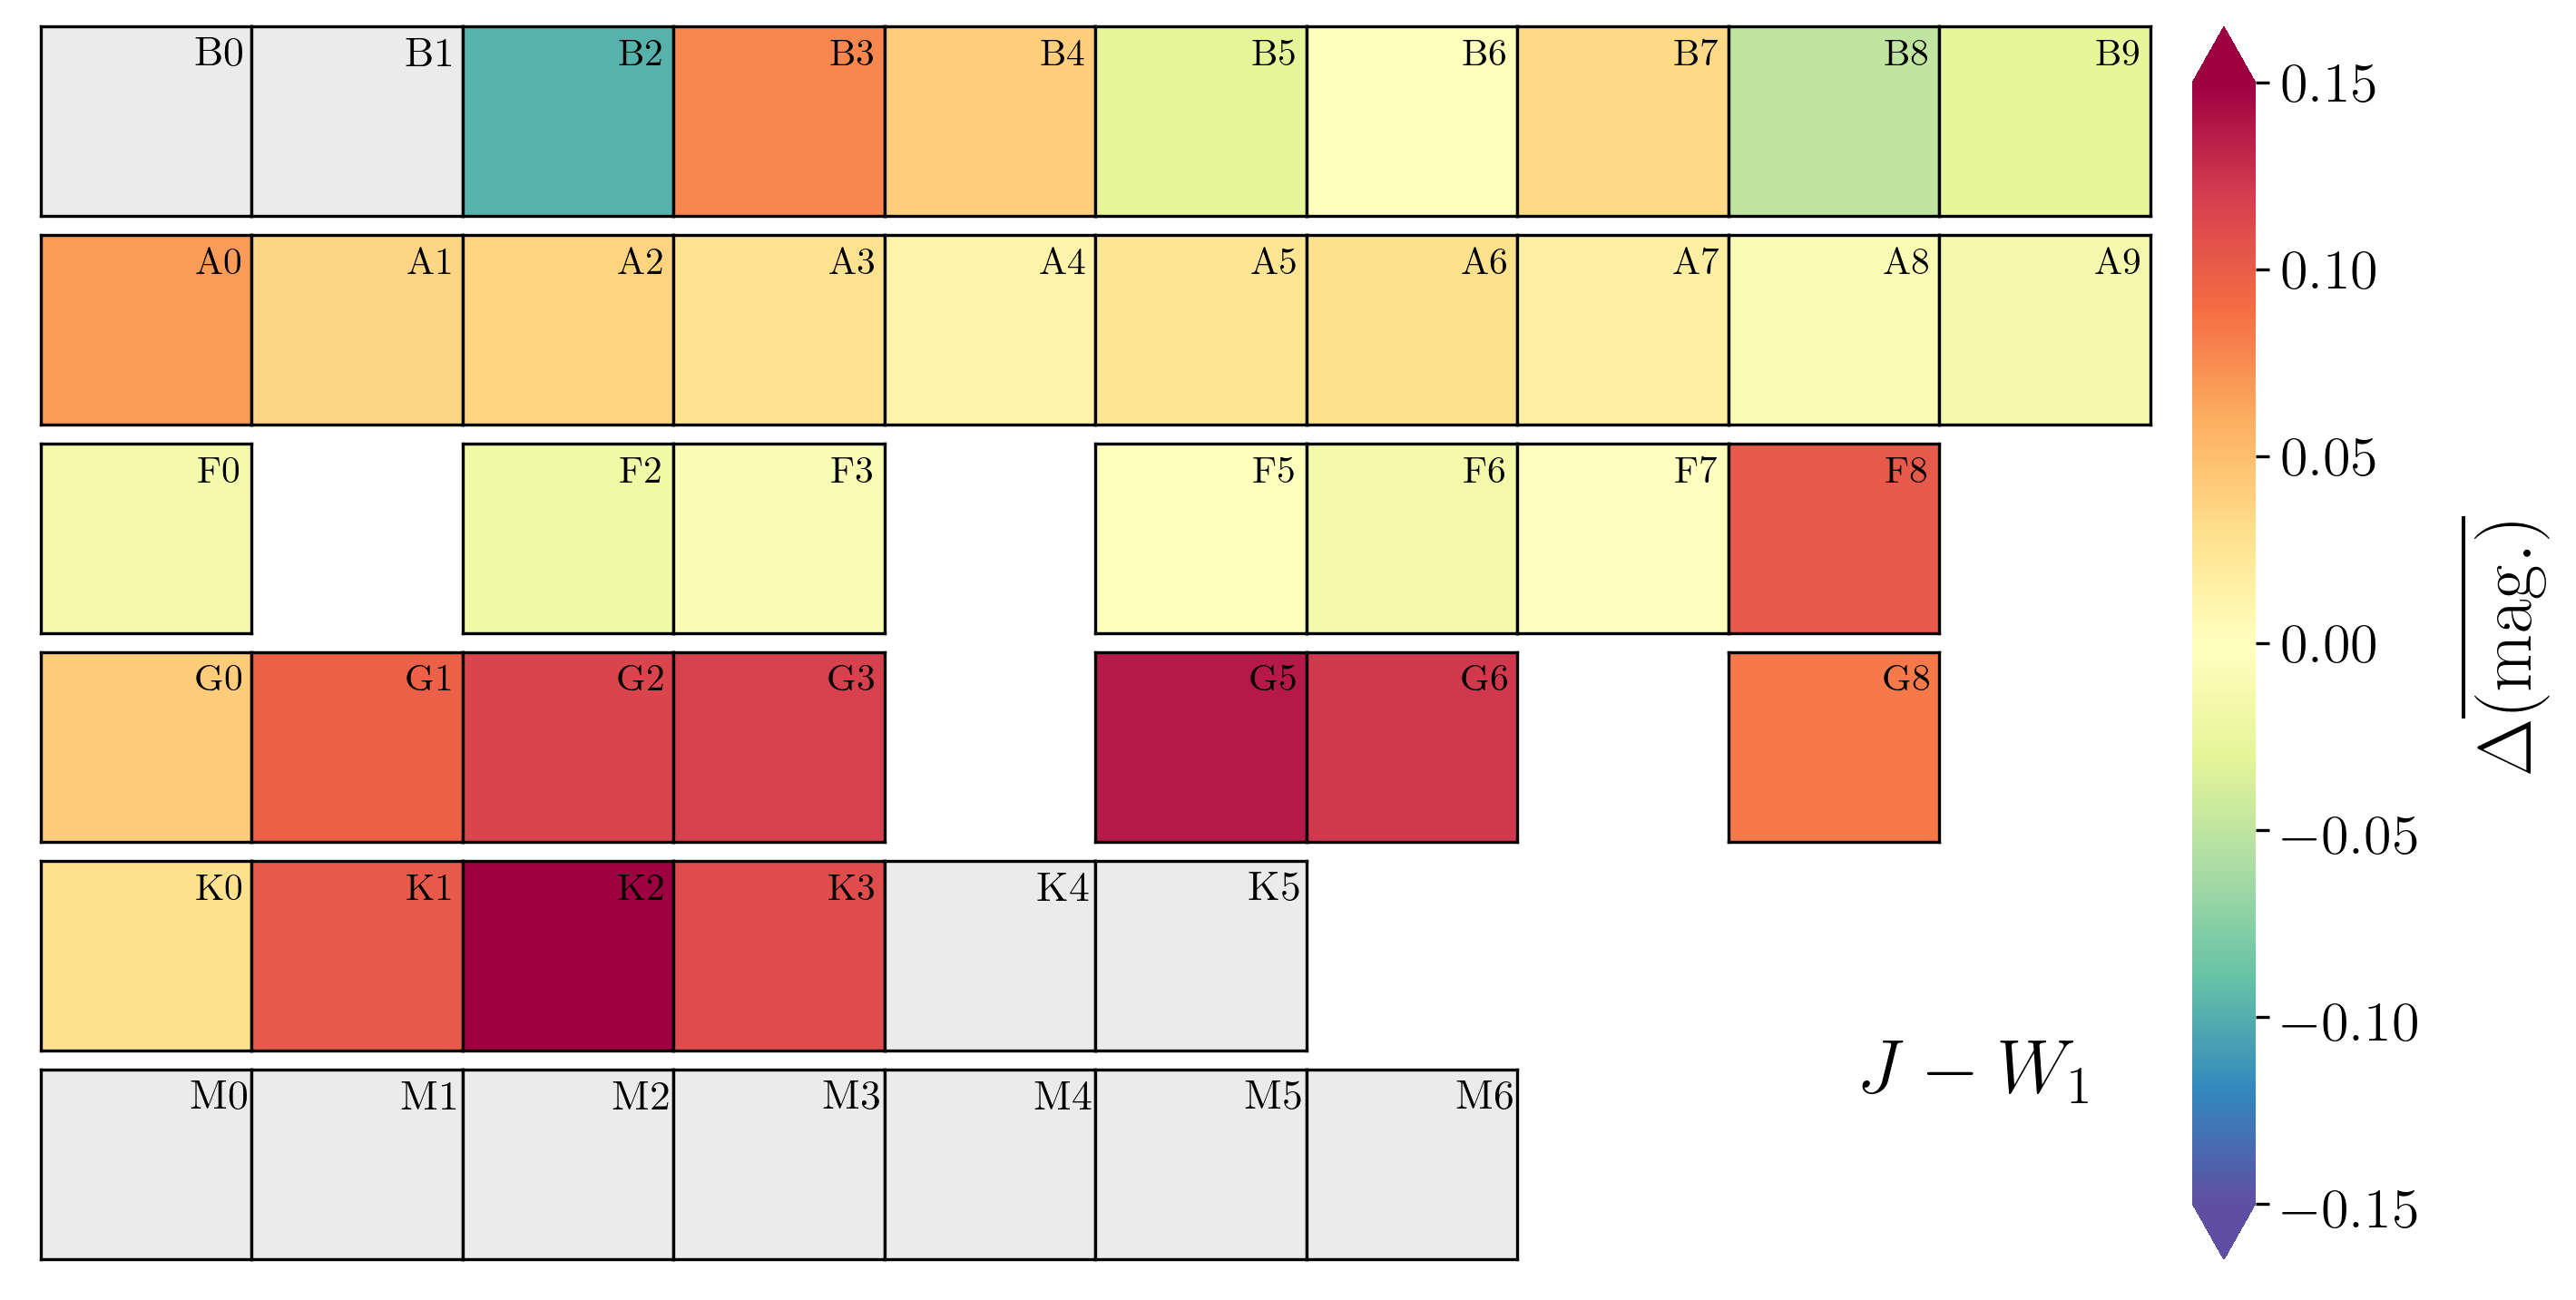
\includegraphics[width=1.0\textwidth,clip=true]{Figures/periodic/periodic-delta_J_W1.png}
    \caption{This figure maps the difference of average color of giants from dwarfs for each spectral sub-type for which we have at least 4 stars in either luminosity group (dwarfs or giants). Giants have the greatest separation from dwarfs for G0--K3 stars. The average separate for these spectral sub-types is $\sim$0.10 magnitude. See Chapter \ref{sec:color_prob_func} on how these averages were calculated. See Appendix C, Table \ref{table:color_avgs} for the average color values and differences of these averages.}
    \label{fig:periodic-delta-jw1}
\end{figure}

\begin{figure}
    \centering
    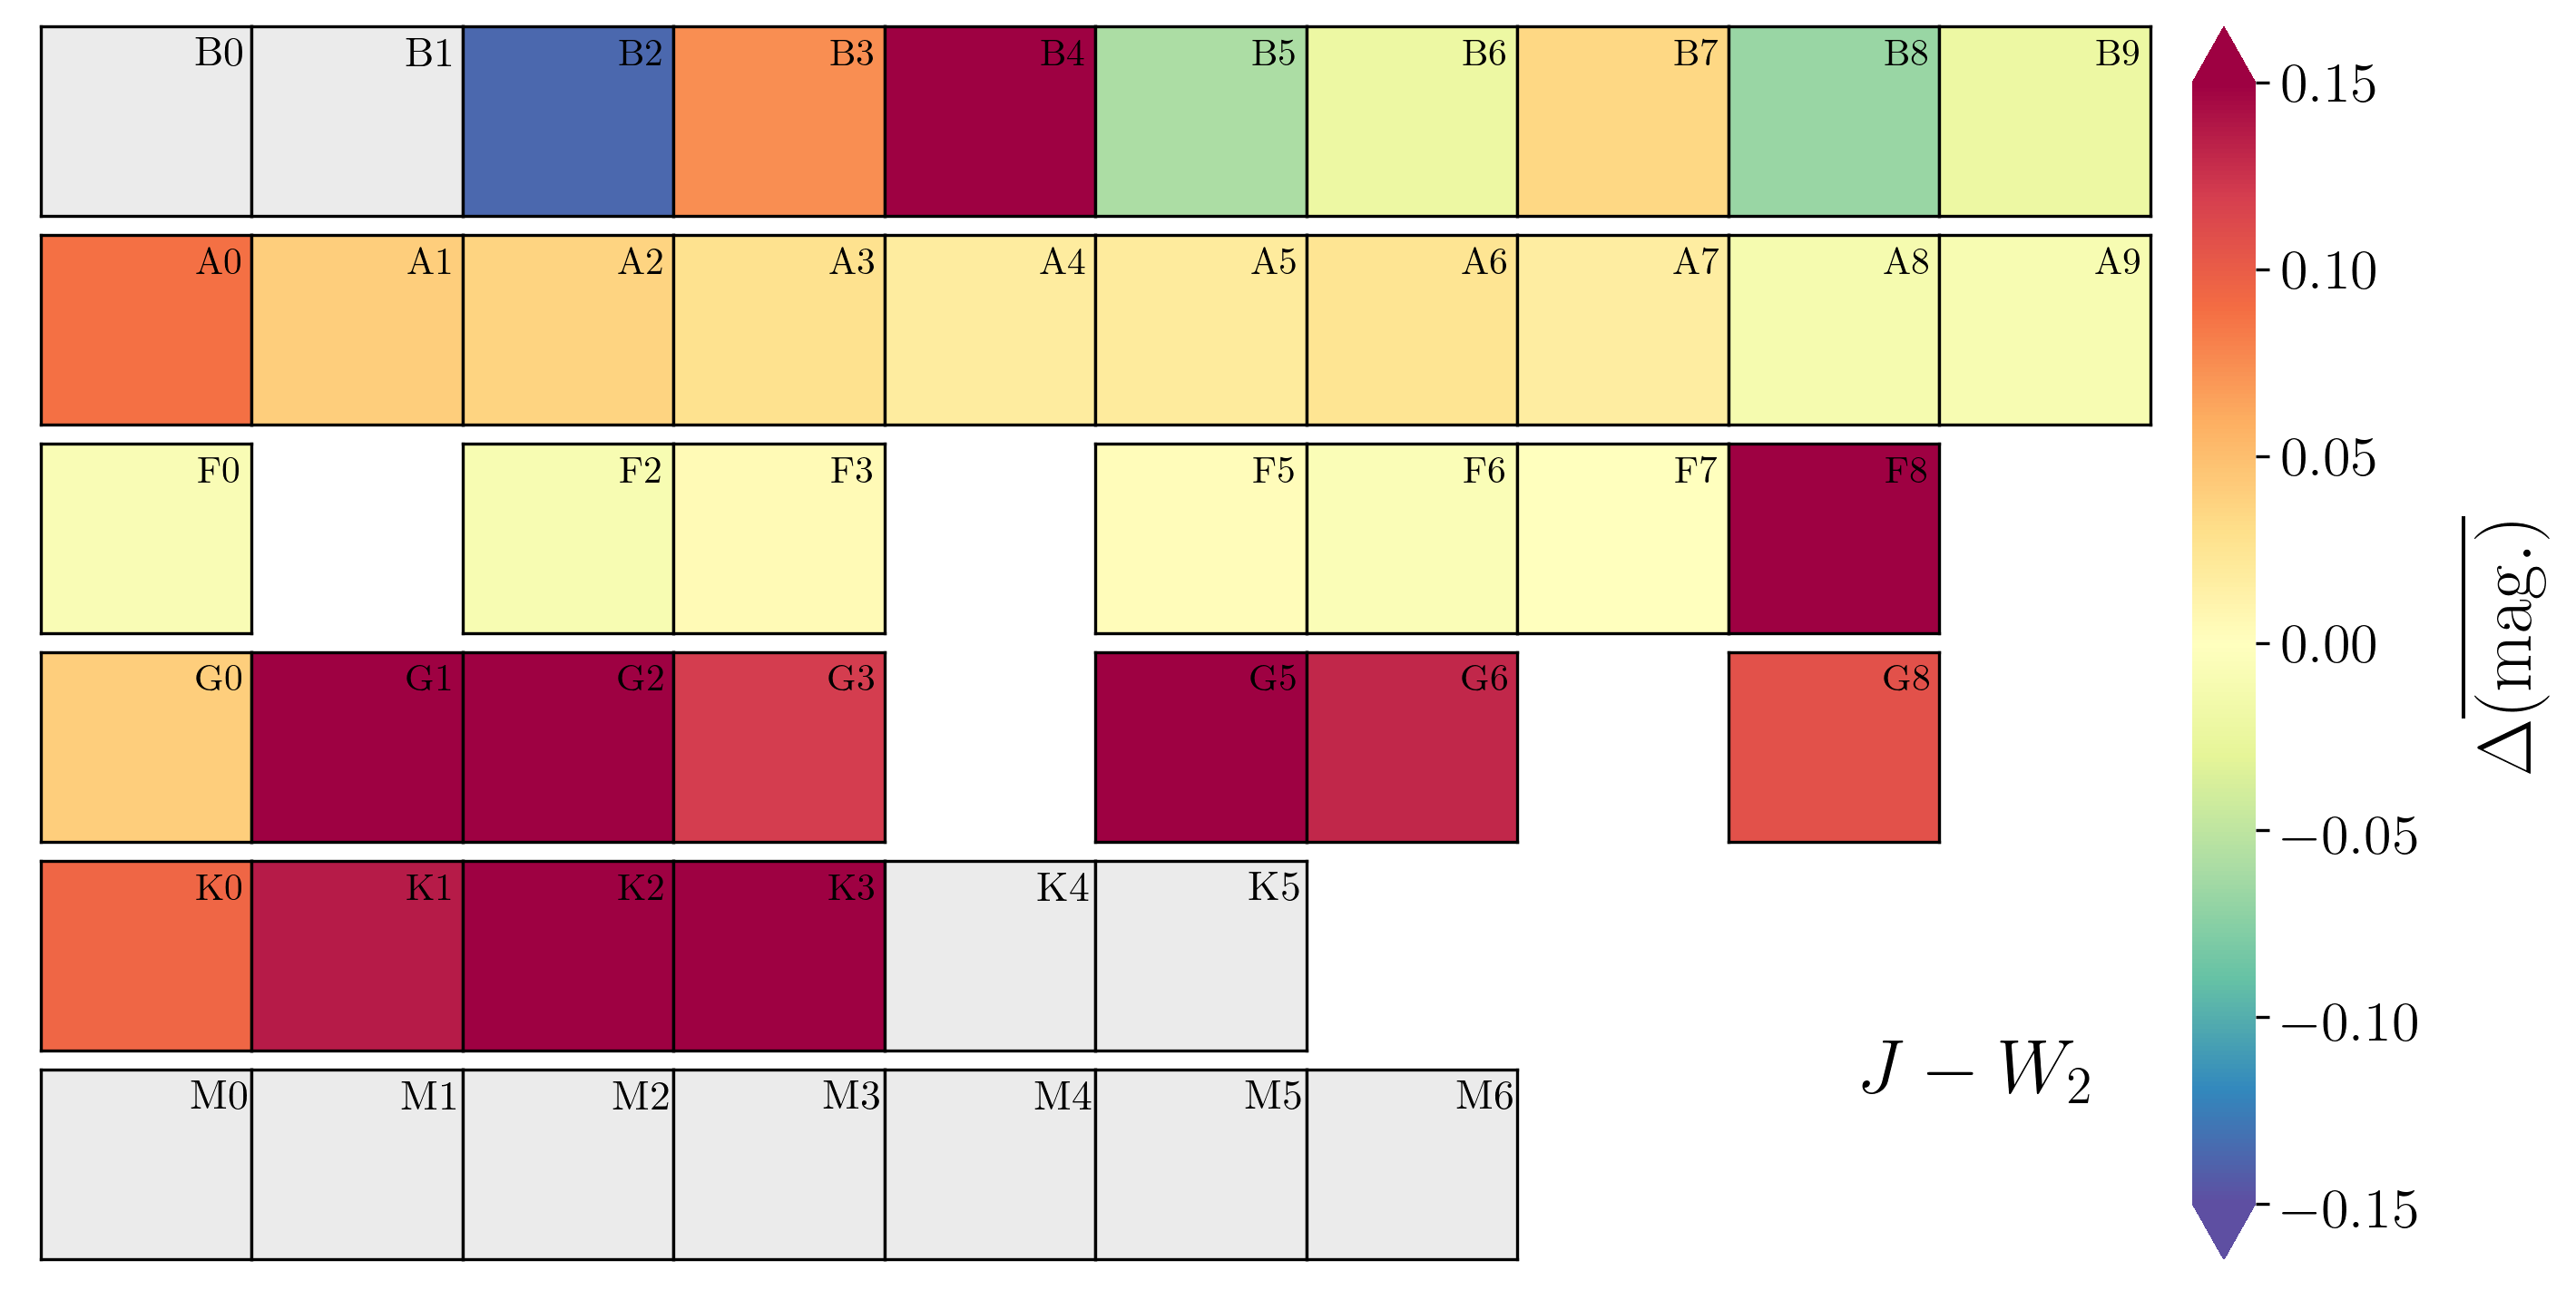
\includegraphics[width=1.0\textwidth,clip=true]{Figures/periodic/periodic-delta_J_W2.png}
    \caption{Same as Figure \ref{fig:periodic-delta-jw1}, but for \jwtwo. The average separate for these spectral sub-types G0--K3 for which we also see the greatest difference (as in $J-W_{1}$) is $\sim$0.14 magnitude. Thus, the color separation on average is greater on \jwtwo than for $J-W_{1}$.}
    \label{fig:periodic-delta-jw2}
\end{figure}
